\section{Introduction}

Neural networks (NNs) and other machine learning (ML) techniques are becoming an increasingly important tool in of modern research process. This is due to their wide application in data-intensive problems, and ability to make progress where prior computational methods have proved otherwise intractable.

The primary method of training ML models involves the construction of a loss function or equivalently a reward function, framing the training process as a high-dimensionality optimisation problem.
In this setting, the parameters of the model are varied such as to minimise the aggregate loss of the model's action, when taken over a large collection of inputs, compared to known corresponding outputs.
Thus it is the loss function that grounds the model in a given problem.
The construction of loss functions varies across applications, but overall they exhibit some general characteristics as will be discussed.

% Cite: https://en.wikipedia.org/wiki/Symplectic_integrator and DT's unpublished paper.
\todo{check with DT about the wording of "canonical symplectic 2-form of the system"}
\SymI{}s are numerical integrators for Hamiltonian systems, which preserve the canonical symplectic 2-form of the system. 
This makes them widely applicable to physical fields such as orbital dynamics and  molecular dynamics, among others.%
\todo{Cite papers, some from DT2, some of my own}%
Consequentially, they will preserve, or near preserve, the constants of motion of a system over a large number of integration steps.

The \SI{} (SI)\cite{tsangSLIMPLECTICINTEGRATORSVARIATIONAL2015} is a non-conservative extension of a symplectic integrator, which enables numerical integration of non-conservative systems. As with the symplectic integrators, this exhibits well-defined bounds in the fractional error of the energy, and other conserved quantities of the system. These are based on the non-conservative action approach developed by Galley \cite{galleyClassicalMechanicsNonconservative2013} and Galley \etall \cite{galleyPrincipleStationaryNonconservative2014}.

\todo{quote types, Maisy says single, maybe smaller sentence also}
Automatic-differentiation techniques are a collection of computational methods for the determination of the derivatives of large classes of \enquote{regular}scientific code, doing so in an efficient and accurate manner. In contrast, the \SI{} is currently implemented using computer algebra systems such as SymPy \cite{sympy}, which represents and works with mathematical expressions symbolically, allowing for the computation of derivatives and integrals. These are general systems and are effective at working with a large range of expressions, but pose limitations when seeking to increase computational speed or to scale up to larger, more complex, physical systems.

In this paper, we focus on taking the existing mathematical framework of the \SI{} and adapting it to use more advanced computational methods. In addition, making it amenable to \autodiff{} which enables a wide class of new applications.
These include scaling to larger systems, for example in molecular dynamics and condensed matter simulations, to its use as the foundation of several physics-based loss functions. These loss functions will evaluated for empirical and theoretical suitability, with the goal that these could be used in the creation of machine learning models which encode physical knowledge and insight, as discussed in the final part of the paper. \todo{Maisy wants to change/qualify insight}

\section{Preliminaries}

\subsection{Lagrangian Mechanics}
\label{sec:lag-mech}

Lagrangian mechanics is a formalism of classical mechanics which places emphasis on the energies and systems of the system and that allows flexibility in the exact variables used to parameterise the system.
As it is traditionally phrased it works to solve the problem of determining the evolution of a physical system, parameterised by $n$ generalised degrees of freedom, represented as the vector $\vb q = \set{q_1, \dots, q_n} \in \R^n$, across the timespan $[t_i, t_f] \subset \R$ from some initially known configuration $\vb q_0 \in \R^n$. This determination is done by constructing a functional,

\begin{equation}
  \label{eq:trad-action}
  S[\vb{q}] = \int_{t_i}^{t_f} L(\vb{q}, \dot{\vb{q}}, t) \rdd t
\end{equation}

where $S$ is known as the action of the system, $\dot\vbq$ is the standard time derivative of the system's path, and $L$ the Lagrangian. The Lagrangian being traditionally made up of two components $T$, the kinetic energy of the system in some configuration at some time, and $V$, the potential energy of the system. These are combined as,

\begin{equation}
  \label{eq:trad-lag}
  L(\vb{q}, \dot{\vb{q}}, t) = T(\vb{q}, \dot{\vb{q}}, t) - V(\vb{q}, \dot{\vb{q}}, t).
\end{equation}

A physical solution is arrived at by then employing Hamilton's principle of least action \cite{goldsteinClassicalMechanics2000} which provides that the physical path, $\vb q(t)$, is the one that \textit{extremises} the functional $S[\vb q]$ as defined in Equation \eqref{eq:trad-action}, ie one where the variation $\delta S$ with respect to any variation of the path $\delta \vbq(t)$ is zero. This equation can be found by solving the Euler-Lagrange equations,

\begin{equation}
	\label{eq:euler-lagrange}
	\frac{\p L}{\p q_i} - \frac{\dd}{\dd t}\frac{\p L}{\p \dot q_i} = 0
\end{equation}

for each generalised degree of $q_i$. To each we can also associate a conjugate momentum $p_i$ and generalised force $F_i$,

\begin{align}
  p_i = \frac{\p L }{\p \dot q_i} \\
  F_i = \frac{\p L}{\p q_i}
\end{align}

such that Equation \eqref{eq:euler-lagrange} reads in line with Newton's second law, $F = \dot{p}_i$.

The focus on symmetries within the formalism comes to the fore however when we consider Noether's Theorem \cite{noetherInvariantVariationProblems1971} which states that every continuous symmetry of the action $S$ has a corresponding conserved quantity. A simple example of this can be seen for degrees of freedom which are said to be \emph{cyclic} in that the coordinate value itself, $q_i$, does not appear directly in the Lagrangian. It can be readily seen from Equation \eqref{eq:euler-lagrange} that if this is the case then,

\begin{equation}
  \frac{\dd}{\dd t}\frac{\p L}{\p \dot q_i} = 0
\end{equation}

which implies that the conjugate momentum $p_i$ is a conserved quantity of the system.

\subsection{Non-Conservative Actions}
\label{sec:intro-nc-actions}

Lagrangian mechanics as discussed applies only to conservative systems. While there exist other extensions to non-conservative systems, notably Rayleigh dissipation functions \cite{struttGeneralTheoremsRelating1871} for simple dissipative functions, we will focus on the method put forward by Galley \etall \cite{galleyClassicalMechanicsNonconservative2013}.

\begin{figure}[t]
  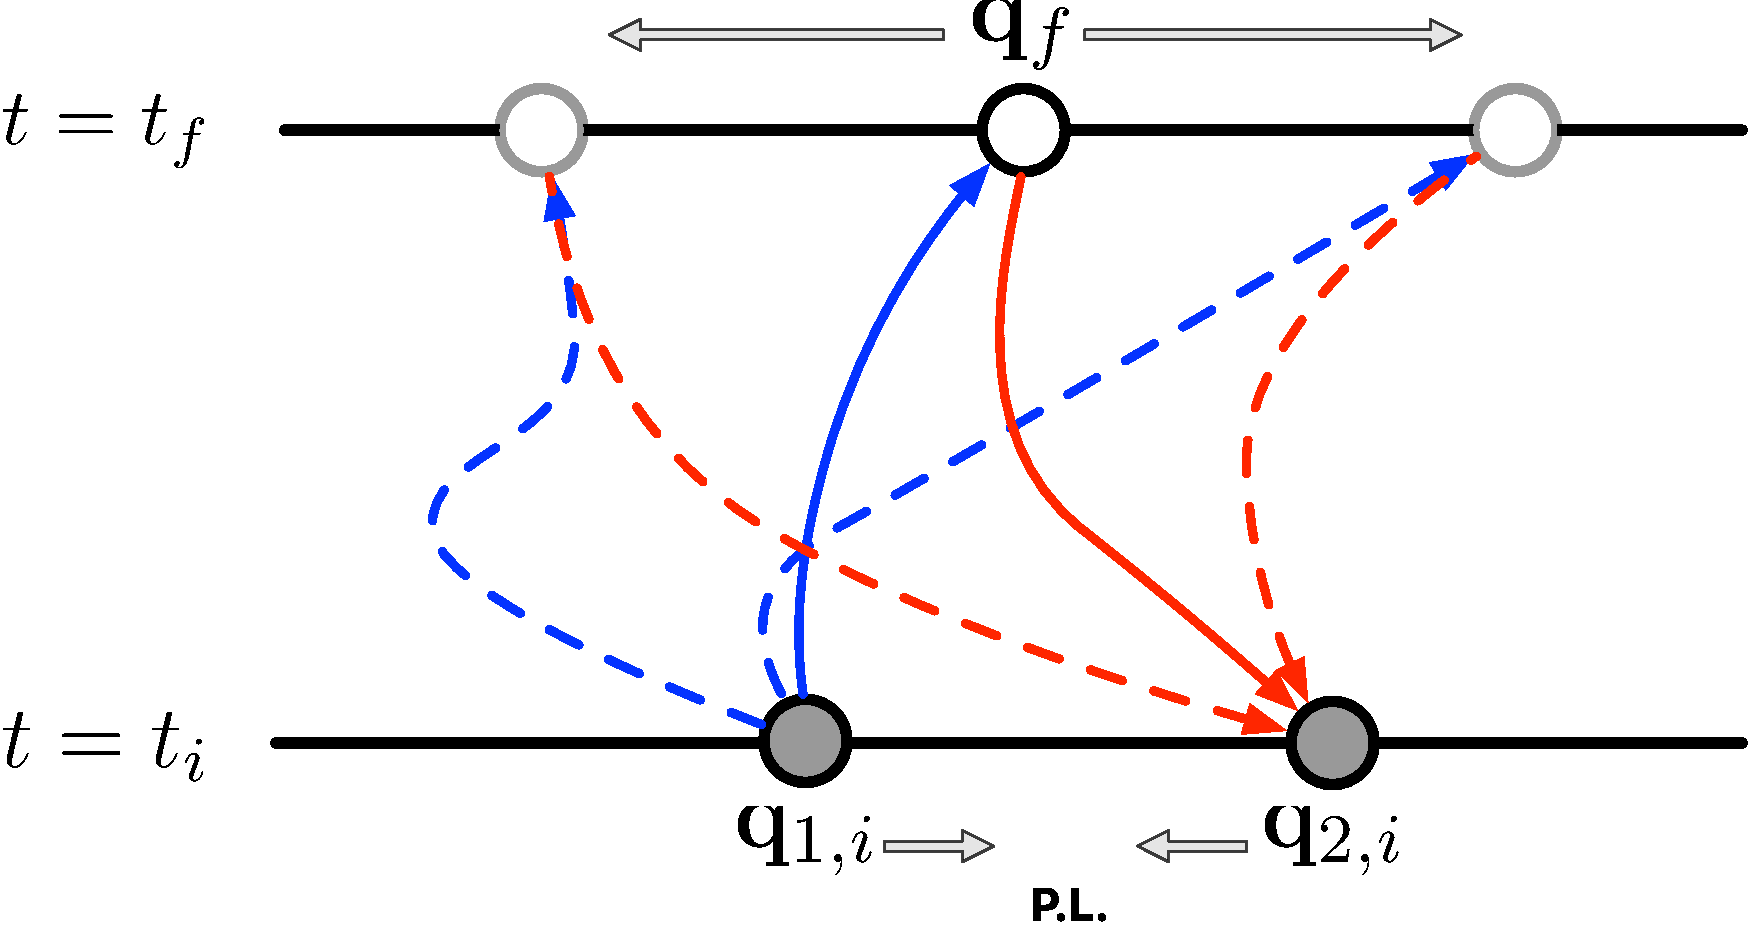
\includegraphics[width=\columnwidth]{figures/qif-two-paths.pdf}
  \caption{A cartoon based on a similar figure from \cite{galleyClassicalMechanicsNonconservative2013} showing the two virtual paths. We can see that the two paths initiate at their respective initial configurations $\vbq_{i,\set{1,2}}$ at time $t_i$ and are connected by the final configuration $\vbq_f$ at $t_f$. This final configuration is unknown and is allowed to vary within the problem (depicted as two alternative values shown in pale either side), depending on the value of $\vbq_{i,\set{1,2}}$. which are fixed during extremisation (displayed in grey). In this manner the problem's boundary resides purely in the $t = t_i$ plane where physical information is known. As shown the physical limit (P.L.) consists of bringing the two virtual paths together such as $\vbq_{i, 1} = \vbq_{i, 2}$.}
  \label{fig:nc-lagrange-virtual-paths}
\end{figure}

This method was originally developed to account for the fact that while we often employ Hamilton’s principle and the Euler-Lagrange equations it produces as an initial value problem, it is formally a boundary value problem in time. To remedy this difficulty we formally double the degrees of freedom of our system into two new virtual paths $\vb q_{1,2}$, with an adapted non-conservative Lagrangian $\Lambda$ given by,

\begin{equation}
  \label{eq:nc-lag}
  \Lambda = L(\vbq_1, \dot\vbq_1, t) - L(\vbq_1, \dot\vbq_1, t) + K(\vbq_1, \vbq_2, \dot\vbq_1, \dot\vbq_2, t).
\end{equation}

The form of this equation, as well as the visualisation shown in \fref{fig:nc-lagrange-virtual-paths}, shows we can consider this doubling as creating two paths, one forwards in time, the other backwards (and hence negative in \eqref{eq:nc-lag}), with both of these paths contribute with terms as the traditional conservative Lagrangian. There is also an additional term $K$, the non-conservative potential, representing a non-conservative coupling between the two paths (if it could be broken down cleanly into a form of $V(\vbq_1) - V(\vbq_2)$or similar, and thus being conservative, then these could be absorbed into $L$ leaving $K = 0$). In this way the system becomes a boundary value problem as needed, with both paths sharing the $\vbq_f$ point as one of their boundaries.

To solve this system we follow in the same form as before, aiming to extremise a new action defined now in terms of $\Lambda$, however crucially we do so in what is known as the \enquote{physical limit} (P.L), where $\vbq_1 = \vbq_2$. This gives the non-conservative Euler Lagrange equation,

\begin{equation}
	\label{eq:nc-el}
  	\left[\frac{\p \Lambda}{\p q_i} - \frac{\dd}{\dd t}\frac{\p \Lambda}{\p \dot q_i}\right]_{\text{P.L}} = 0
\end{equation}

In practical considerations it is often useful to alter our choice of variables to instead be $\vbq_+ = {(\vbq_1 + \vbq_2)}/{2}$ and $\vbq_- = \vbq_1 - \vbq_2$. This reduced our P.L. condition to simply $\vbq_- \to \vb 0$. Note that only the Euler-Lagrange equation involving differentiating wrt. $\vbq_-$ survives. We can of course also define a corresponding conjugate momenta,

\begin{equation}
  \pi_{\mp, i} = \frac{\p \Lambda}{\p q_{\pm,i}}.
\end{equation}

A corresponding form of Noether's theorem can be shown to hold for these non-conservative systems where the Noether currents evolve in time due to the effect of the non-conservative coupling potential $K$ \cite{galleyPrincipleStationaryNonconservative2014}. There one can also find a more complete explanation of the process described above, along with a rigorous derivation.

\subsection{The \SI}
\label{sec:intro-si}

The \SI{} is an extension of a symplectic integrator to non-conservative Lagrangian mechanics, symplectic integrators being those which preserve the canonical symplectic 2-form of the system $dp \wedge dq$, and thus preserve many desired properties during integration.

Hence, to understand the \SI{} method we first consider the application of a symplectic integrators to a traditional conservative system\footnote{This explanation takes its path from an unpublished paper by Tsang \etall \cite{tsangVariationalSymplecticIntegrators}}. As before consider a system with $N$ degrees of freedom represented by some $\vbq \in \R^N$, governed by some Lagrangian, $L(\vbq, \dot{\vbq}, t) \in \R$.

With this set up we now choose to apply two successive procedures to our extremal path $\vb q(t)$: first piecewise breakdown and then discretisation of the action itself. It is this ordering that differentiates this symplectic method from more traditional integrators such as Runge-Kutta \cite{devriesFirstCourseComputational2011} which solve similar systems by discretising the final equations of motion themselves rather than the action, before equations of motion are formed.

To start we break the trajectory down piecewise into a collection of $M$ sub-paths $\gamma_{n \in [M - 1]}$ where $[A] = \set{0, \dots, A}$, each defined on some portion of the whole timespan $[t_n, t_{n + 1}] \subset [t_i, t_f] \subset \R$ such that they cover it completely with overlaps only at the boundaries of the intervals. These together are such that the there is the correspondence,

\begin{equation}
\label{eq:pw-traj}
	\vb q(t) = \begin{cases}
		\gamma_n(t) &\text{for~} t \in [t_n, t_{n + 1}]
	\end{cases}
\end{equation}

between the total path and sub-paths for all $t \in [t_i, t_f]$. These paths define a collection of points $\vb q_{n \in [M]}$ which are their mutual values at the piecewise break points (which we required to be equal) and the initial and final values for $n = 0$ and $n = M$ respectively.

As each piecewise curve constitutes in and of itself a physically attained trajectory we can state that any path $\vb{q}(t)$ which extremises the action for the whole timespan, must also extremise each piecewise portion, and visa-versa. 

This does not bring us closer to a numerical solution directly but allows us to freely split our integral domain as needed without loss of accuracy, and thus limit the error of our numerical-integration method which will necessarily increase with the number of time-steps or their size.

We now turn to the discretisation method itself. This is done using the Galerkin-Gauss-Lobatto (GGL) quadrature method of order $r \in \N_0$\cite{tsangSLIMPLECTICINTEGRATORSVARIATIONAL2015, farrVariationalIntegratorsGravitational2007} which approximates the integral from $t_n$ to $t_{n + 1}$ using the intermediary points

\begin{equation}
  t^{(i)}_n = t_n + (1 + x_i)\frac{\Delta t}{2}
\end{equation}

% NOTE: Orders defined here

where $i \in [r + 1]$ and $x_i$ are the ordered roots of the the derivative of the $(r + 1)$th Legendre polynomial $P_{r + 1}$ and $\Delta t = t_f - t_i$. For a given choice of $r$ this provides slimpletic maps that are accurate up an order $2r + 2$\cite{tsangSLIMPLECTICINTEGRATORSVARIATIONAL2015}. In turn we also define $\vbq_n^{(i)} = \vbq(t^{(i)}_n)$ to be the value of each sub-path at each $t^{(i)}_n$, which we label interior points. This process can be seen visually in \fref{fig:si-process}.

\begin{figure}[t]
  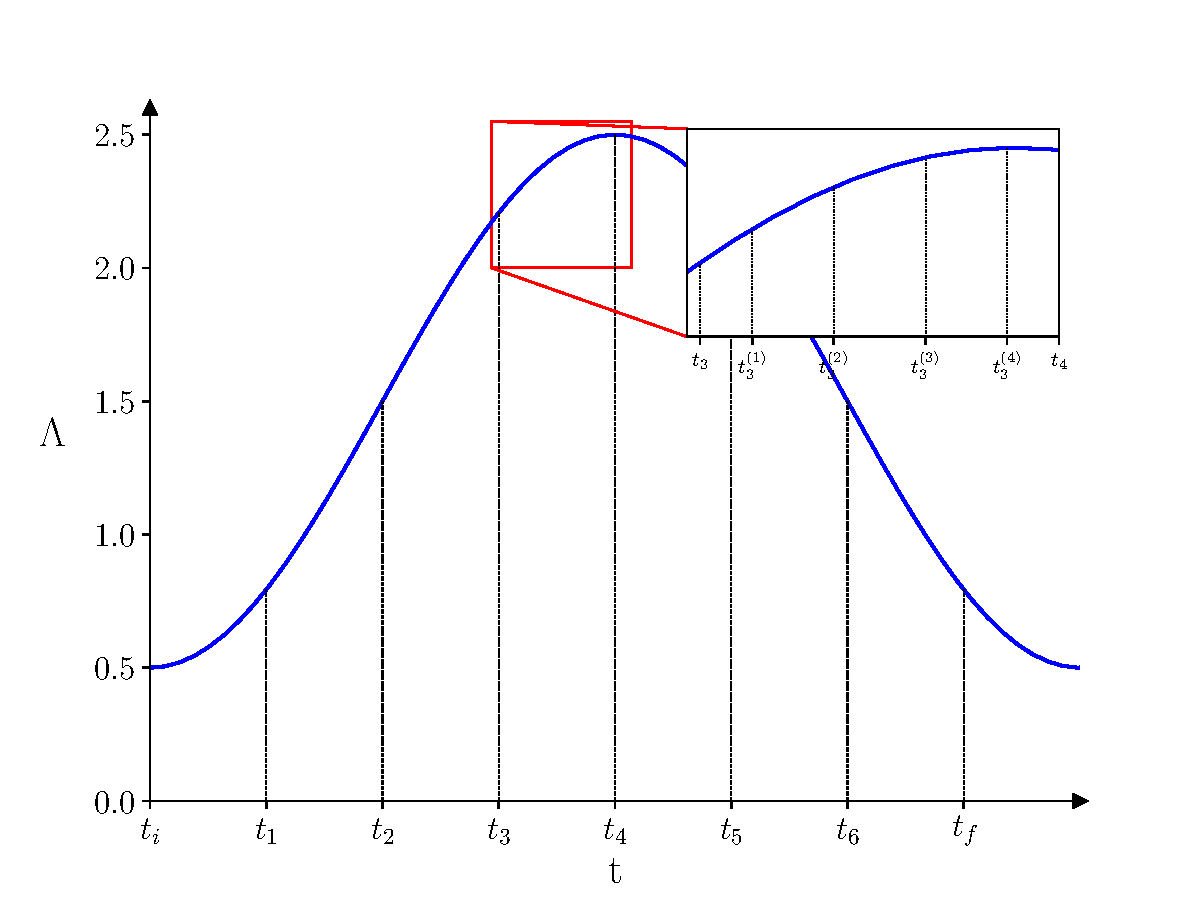
\includegraphics[width=\columnwidth]{figures/si-process.pdf}
  \caption{A depiction of the piecewise breakdown and then discretisation of the action. Each $t_n$ represents shows the action over a subpath $\gamma_n$. In addition we focus on the sub-path spanning $[t_3, t_4]$ showing the interior times $t_{3}^{(i)}$ for $r = 4$.}
  \label{fig:si-process}
\end{figure}

We now approximate the path of the system within this quadrature using the associated cardinal functions for the GGL quadrature, labelled $\phi(t)$, as \(\vb q(t) = \phi(t) + \Or((\Delta t)^{r + 2})\). These provide a suitable approximation for the path derivative $\dot{\vb q}$ by the use the derivative matrix,

\begin{equation}
\label{eq:dij}
  D_{ij} = \begin{cases}
  	\dfrac{(r + 1)(r + 2)}{2\Delta t} &i = j = 0 \\\\
  	-\dfrac{(r + 1)(r + 2)}{2\Delta t} & i = j = r + 1 \\\\
  	0 & i = j \land i \notin \set{0, r + 1} \\\\
  	\dfrac{2P_{r + 1}(x_i)}{P_{r+1}(x_j)(x - x_j)\Delta t} & i\neq j
  \end{cases}
\end{equation}

which provides that,

\begin{equation}
  \dot\phi(t_n^{(i)}) = \sum_{j = 0}^{r + 1} D_{ij}q_n^{(j)}.
\end{equation}

In turn this allows to express the integral as,

\begin{equation}
\label{eq:discr-action-1}
  \int_{t_n}^{t_{n + 1}} L(\vb q, \dot{\vb q}, t) \dd t \approx \sum_{i = 0}^{r + 1} w_i L(q_{n}^{(i)}, \dot\phi_{n}^{(i)}, t_{n}^{(i)})
\end{equation}

where the label the approximate expression $L_d^n$ and where $w_i$ are the quadrature weights given by

\begin{equation}
  w_i = \frac{\Delta t}{(r + 1)(r + 2)(P_{r + 1}(x_i))^2}.
\end{equation}

Equation \eqref{eq:discr-action-1} strung together across the different piecewise sub-trajectories defined in equation \eqref{eq:pw-traj} gives us the total discretised action of the system, shown in Equation \eqref{eq:discr-action-2}, that sets symplectic integrators apart from their more general counterparts,

\begin{align}
\label{eq:ldn}
L_d^n &= \sum_{i = 0}^{r + 1} w_i L(q_{n}^{(i)}, \dot\phi_{n}^{(i)}, t_{n}^{(i)}), \\
\label{eq:discr-action-2}
  S_d &= \sum_{n = 0}^{M} L_d^n.
\end{align}

From here we then extremise this discretised action with respect to the mutual and interior points to obtain the equations of motion of the system as,

\begin{gather}
	\frac{\p L_d^{n-1}}{\p q_n} + \frac{\p L_d^{n}}{\p q_n} = 0 \\
	\label{eq:Ld-interior-eom} \frac{\p L_d^{n}}{\p q^{(i)}_n} = 0.
\end{gather}

This first equation can be simplified further into two equivalent definitions for the discrete momentum \(\pi_n\),

\begin{align}
	\label{eq:pi-n} \pi_n &= -\frac{\p L_d^{n}}{\p q_n} \\
	\label{eq:pi-n+1} \pi_{n + 1} &= \frac{\p L_d^{n}}{\p q_{n + 1}}
\end{align}

and a continuity constraint that they both be equal at these mutual overlap points $\vbq_n$ in the same manner as we required for $\vbq_n$ itself. Together Equations \eqref{eq:Ld-interior-eom}, \eqref{eq:pi-n} can be solved to determine the values of $\vb q^{(i)}_n$, from which Equation \eqref{eq:pi-n+1} provides a form for determining $\pi_{n + 1}$.

This derivation is provided in terms of the traditional conservative Lagrangian $L$ however can be readily adapted to the non-conservative Lagrangian formalism discussed in \sref{sec:intro-nc-actions} by considering instead the non-conservative Euler-Lagrange Equation \eqref{eq:nc-el}, in effect substituting $L$ for the non-conservative Lagrangian $\Lambda$ and $\vb q_n$ for $\vb q_{n, -}$.

Continuing the consideration of Noether currents from prior sections, it can be shown that the continuous symmetries of the conservative action evolve as due to this now discretised $K_d$. It should be noted that GGL discretisation does not preserve time-shift symmetry, and hence energy is non conserved under the operation, however we will show, in line with previous work \cite{tsangSLIMPLECTICINTEGRATORSVARIATIONAL2015}, that the fractional error is generally bounded over the integration.

\subsection{Physics Informed Neural Networks}
\label{sec:intro-pinn}

Physics informed neural networks (PINNs) are neural networks which include physical knowledge in their training processes \cite{raissiPhysicsInformedDeep2017}.
Their most common application is in solving partial differential equations (PDEs) \cite{luDeepXDEDeepLearning2021,mengCompositeNeuralNetwork2020} where we take physically derived knowledge of the system as a prior in training and train the neural network with a loss function incorporating the residuals from the initial and boundary conditions (loss functions will be discussed in more depth in \sref{sec:intro-lf}).

Neural networks more generally are a collection of linear and non-linear components composed together to form complex non-linear functions. At their base level the linear components can be expressed as the simple linear equation \(\vb{y} = W\vb{x} + \vb{b}\) where $W$ is a matrix of weights for this component and $\vb{b}$ the biases. The non-linear components are functions such as sigmoid or $\tanh$ which stop collapse to linearity for the whole composition, allowing for non-trivial behaviour. These weights, biases, and other variables within the model constitute the model's \emph{parameters}.

This composition is useful as it can be shown that, with sufficient complexity, these forms are dense in the space of Borel measurable functions and hence can take the place of almost any physical function or mathematical procedure \cite{hornikMultilayerFeedforwardNetworks1989}.

\subsection{Loss functions}
\label{sec:intro-lf}

The primary method of training ML models involves the construction of a loss function or equivalently reward function. This frames the training process as a high-dimensionality optimisation problem. In this setting, the various parameters of the model are varied such as to minimise the aggregate loss of the model's action over a large collection of inputs when compared to known corresponding outputs. It is thus the loss function that grounds the model in a given problem. Their construction varies but they exhibit some general characteristics as will be discussed.


Loss functions are the primary learning method of neural networks and, in PINNs, act as the place where physics steps in to connect our computational model to reality. As mentioned they are used to construct a high-dimensionality optimisation problem where we seek to minimise arbitrary loss value computed from the parameters, aggregated over a large collection of inputs when compared to known corresponding outputs.

A loss function traditionally takes the form, $\mathrm{loss} = f(y_{\text{true}}, y_{\text{pred}})$ where $f$ is some chosen function and $y_{\text{pred}}$ and $y_{\text{true}}$ are both real vectors in the output space of the model, representing the known models output and the known true output respectively.

Loss functions in PINNs are often comprised of two components. First there is the prediction or physical loss which may, as mentioned, be made up of the residuals of the model under PDE, boundary, and initial conditions of the system. Secondly there a regularisation loss term which helps to penalise overfitting to the training data, expressed as \enquote{complexity}, within the model. This might be implemented as an $L^2$ of a vector containing all parameters of the model.

Optimising this loss function can be thought of as a traditional minimisation problem, with common choices of the method being Stochastic gradient descent and Adam \cite{kingmaAdamMethodStochastic2017}. These impose various requirements on the loss function, for example generally that it is differentiable \footnote{Although methods exist for non-differentiable functions \cite{daubechiesIterativeThresholdingAlgorithm2003}.} and benefits from other properties such as higher-order differentiability, Lipschitz continuity, and convexity \cite{sraOptimizationMachineLearning2012}. The rate at which these methods apply gradient based updates is determined by a provided learning rate, which will often be varied through training to quickly move towards minima during the initial stages, then tuned down to avoid \enquote{jumping} over the minima as we close in on the optimal solution.

\subsection{Lagrangian Embeddings}

To work with non-conservative Lagrangians $\Lambda$ computationally, for example as the output of a PINN, or one of the inputs of a loss function, we must define some mapping from a collection of real numbers, to a form of $\Lambda(\vbq, \dot\vbq, t)$. This can be thought of as a function,

\begin{equation}
  E: \R^n \to \mathbb{L}
\end{equation}

where $E$ is known as an \enquote{embedding function} and $\mathbb{L}$ is a subset of the overall function space of possible $\Lambda$ values. 
The choice of embedding necessarily restricts and dictates the systems which the system can deal with, and hence our choice of embedding is crucial, discussions of different embeddings used in this paper can be found in \sref{sec:eg-sys}.

There are two broad approaches to designing an embedding function. Either one can be chosen to represent a specific system by its physical parameters, or a more broad class of systems can be represented by some arbitrary function approximation scheme such as Fourier series or Taylor expansion around a point.

It should be noted that these embeddings often will not have a unique correspondence with physical Lagrangians, ie the map is not injective up to physical behaviour. This has implications for optimisation in creating multiple minima as will be discussed.

\subsection{Automatic-Differentiation, XLA, and Google's JAX}
\label{sec:intro-autodiff}

Automatic-differentiation is the process of computing the differential of \enquote{regular} code with respect to one or more of its arguments. Google's JAX library \cite{jax2018github} contains one implementation of this in Python which works by passing \enquote{tracers} into the Python code that record the actions done to them such that an overall differential can be calculated.

JAX also incorporates the XLA (Accelerated Linear Algebra) library \cite{openxla-xla} where it uses similar tracing methods to translate a restricted, but large, subset of Python code into a series of low-level efficient operations which can be executed at speed on the GPU or CPU.

These two technologies together show great promise in the fields of machine learning and physics simulation as they allow for code that would previously have to be written in low-level languages such as C or C++ to be expressed in Python with significantly reduced overhead at runtime, and easier use by researchers.
